\chapter{Proposed Solution}
\label{cha:proposal}
In this chapter we explain how we can solve the scenarios which we explained in previous chapter.
We introduced seven different scenarios, three of them for linear operations and three of them for non-linear
ones, and one mixed operation type. We begin with the most basic scenario, solving a data intensive operation
which requires one dataset. Then we will extend it to accept more datasets and we will solve them. We will
cover only solving linear operations and non-linear operations will be left for further work.

\section{Big Picture}
To make it easier to consume all this text we will make an effort to show a big picture of our design beforehand. Here it is.

There would be multiple computers, our application installed on each of them. This machines do not depend on each
other to operate. Each of them runs the same program instance as others. Each one has the same set of services that
other instances and users can call. Each instance has a number of datasets. These peers will exchange knowledge of
existing datasets with each other. Each instance contains at least two distributed internal structures,
we call them \textit{stores}, these are similar to distributed key/value stores.
One store for operations, and another one for datasets. When an instance receives a service call for an operation, it
will store some basic information and identification about it inside its operation store. This store automatically will
inform other peers about these changes, so others will have the same knowledge afterwards.

Upon an incoming request, an instance would be able to accomplish the task alone, only if it has access to datasets locally.
Otherwise it will do nothing and will simply ignore it. But since the operation store will distribute this information
seamlessly, any other peer has the opportunity to launch the operation if they have the desired data, if it is not the case
they will only update their internal store and do nothing. But if they had the data, they would run the desired operation
and would update the state of the operation to a meaningful one, such as \textit{processing}, and would distribute it
accordingly to inform others about the new state of this operation.

In case of a mixed operation the receiver will break it into smaller operations and will self-launch them accordingly and
will register a meta operation and will assign the aforementioned smaller operations as sub/child operations. We will
also register this meta operation into the internal operation store and it will then automatically distribute it like any other
operation. This way, we have similar behavior with simple and complicated operations and we use the same interface to interact
with them.

In case of operations which have child operations there would be a need to aggregate the result of sub operations.
This would be done in a seamless way as well. We will introduce a \textit{collector} peer which will randomly take control
and collect the results.

When an operation is done, the result dataset will be given to the internal distributed dataset store of the responsible
peer - the peer which is running it - and it will be stored in a backend storage but the unique identifier of the dataset
will be distributed and other peers will get the knowledge of a new dataset and the container peer respectively. 
To query results users have to use the operation id that they have received upon the initial service call. 

This way we can apply a collaboration technique to a number of autonomous peers. 
This design allows us to have peers which are able to work independently, 
but meanwhile are member of a larger network of peers and participate in accomplishing larger tasks.

We will cover these in more detail during this chapter.

\section{Basic Design}
The basic idea that we will follow in this chapter, relies on breaking the operations into smaller units which
we can solve them in one step, such as only one operation or service call. 
In our design the simple operations are the building blocks for mixed ones.
We build them on top of the atomic units, which we know how to solve them.
This idea has the advantage of allowing us to reuse our work and decrease the complexity of implementing
more complicated operations. However we would have increased complexity in messaging parts.

We assume that we have the information about the datasets
available on all machines i.e. in form of a distributed table
with entries containing the node address and dataset id. Based on this
information the application can decide if it has the required data or
not. We will explain this in detail later in this and next chapter.

Based on this algorithm the application implicitly delegates operations to the other 
nodes (instances of the same program), where the data is available. 
It would be a non-blocking service call, 
just like signaling others about an incoming request.
Along with any operation change, the distributed workflow manager will synchronize the information among the peers.
Any change in datasets in any collaborative node will also be synchronized with peers and will be added to 
a distributed list.

Here is a short definition of operations from design point of view:

\begin{itemize}
\item{Simple Operation} Any operation that has only one input dataset. We solve these.
\item{Complex Operations} Operations with more that one input dataset. We turn them into simple operations and then we solve them.
\item{Mixed Operation} Any operation that has another operation as input. We turn them into simple and complex operations and
then we solve them accordingly.
\end{itemize}

\subsection{Break and conquer - recursive call}
This is the high level algorithm that we are using in this work. We break operations into smallest possible operations
and we implement them. Then we build other operations using these small units. For example we solve scenario number one, as
discussed in chapter~\ref{cha:analysis} to run one single operation on a single dataset.
In order to run it successfully we need to find the corresponding dataset and in case it is not available locally we have
to launch the operation on the node which has it. Then when we come to scenario number two, i.e. applying the same operation
on two datasets we break it into two smaller units, and one \textit{meta operation}.

After having two smaller operations and one meta operation, we launch the smaller operations implicitly. Actually we break
scenario number two into two instances of scenario one and one meta operation to observe the overall process. The implementation
of this process will be presented in the prototype.

\subsection{Non-blocking calls}
We base our design on non-blocking service calls. This means all the calls in our system would be asynchronous.
When a user calls a service, she would instantly receive an id, instead of being blocked for the real result.
The rationale here is because of possible long-execution times in our use cases. 
One needs to think of a service call in our design as \textit{request submission}. 
Not only the interaction between user and peers is asynchronous but the inter-peer service calls follow the same path.
Any service call regarding running an operation would be non-blocking and will result in an unique identifier.

\subsection{Dataset identification}
When a user or peer wants to submit a request for an operation, they would not provide a real dataset as input.
They would instead provide the unique id of a dataset existing on our network of collaborative peers.
Then our system, i.e. the peer who has received the request, will make a look up at its internal dataset store to see if it
has the dataset locally or not.
This will happen in the pre-processing step. 
In any case a signal will be dispatched to other peers about the new operation.
The nature of these signals are also non-blocking.

\subsection{Distributed operation}
To realize the above mentioned method, we need to distribute any single operation. To achieve this we assign one unique id
to every incoming operation. This will happen before doing any real work on the request. In our prototype we have implemented
this with \textit{decorators} in Python programming language. 
From this point of time, 
the operation will be known and tracked with this id. One can imagine this as a ticket which
allows monitoring and tracking every change made to an operation while that operation exist in our system. 
Apart from id we will store name of the operation and its input datasets. 
This will allow us to relaunch this operation in case we need to. 
The store that keeps this information is distributed among all participating nodes. 
Any further information such as result dataset ids will be attached to this store during the process. 
There are concerns running a distributed store that needs further attention and 
we try to cover them in further discussions.

\subsection{Distributed store}
We will use this term many times in the next sections, therefore we have to explain it.
Basically we talk about a simple key/value storage. 
Currently the storage mechanism is not important for us, it could be memory or anything else.
This stores are like dictionaries, the keys would be the unique identifiers.
Either id of an operation or id of a dataset. 
Then we will store further information about that object as the value for that key.
We will take advantage of very simple structure to make it easy to be exchanged among peers.

From one side, these stores would be simple repositories to read/write key/value pairs.
This simplifies dependent parts.
From another point of view these stores are distributed objects, but not really.
The keep sending signals about any change in their internals.
These signals will be caught and handled by another component respectively.
The other component will then signal other peers about certain changes that has been happened in this store.
Other peers then will catch this message and will unpack the message and will update their own stores.

This way with minimum coupling we would have a distributed storage which its distributed nature is hidden from
the objects which need to use it.

\subsection{Messaging}
To maintain a network solution we utilize messaging to have peer-to-peer communication. 
We define a number of different message types known to the system. 
Upon arrival of each message type the peer will take corresponding actions.
There are a few message types that are important during this chapter and we introduce them here.

\subsubsection{Delegation call}
Used when a peer asks other to run an operation instead of it.
Other peers will run the requested operation if they have the desired data and will update
the distributed stores as a consequence.

\subsubsection{Operation news}
This happens when a peer wants to inform other peers about a change in its operation store.
Other peers will only update their store respectively.
This message will not cause others to run an operation, 
but this will cause the collective peer to take further actions if required.

\subsection{Meta operations}
Nature of simple operations is simple. 
An operation either will be handled locally or a dispatched signal will be handled
by a peer who has the requested data. 
The status and result dataset id will be stored inside the operation store under the operation's unique id.

As soon as it comes to next scenarios this simplicity vanishes. 
Then we have to deal with multiple operations under one initial request from users.
We have decided to repeat the same structure for operations with one or more datasets.
Therefore in pre-process we check the number of inputs and we create the same number of
smaller operations. 
This is only for linear operations, as we will not cover non-linear operations.
Nevertheless, an input could be an operation call in case of mixed operations.
In this case again we go back to our main patter, \textit{break and conquer}. 
We create a meta operation and we store it. 
We create sub operations for \textbf{level one} operations and we will store its id 
in our meta operation as child operation. 
The same story will happen subsequently for any sub operation as well. 
Meaning that those might also create their own sub-operations and so on.

To better understand this structure think of how method calls work in programming languages.
A programmer can call functions and pass other function calls as input arguments.
The runtime will begin to execute each function call and will use a stack to restore
the last execution point to continue from there after finishing the nested call.
We apply the same mechanism but in a distributed and non-blocking way.

\subsection{Collectors}
In last part we discussed meta-operations. 
But who will be responsible to aggregate the result of these small operations spread all over the network? 
Here we introduce a new role for a peer, \textit{collector}. 
During the pre-process phase, where we create sub-operations we randomly assign
a flag for one of sub-operations to indicate that it should collect the results. 
That peer - which is yet unknown - apart from running its part of the meta operation,
will take an extra responsibility. That is, it would check frequently to see if the
sub-operations are done. As soon as the sub-operations are done, it will
launch the target function, bypassing the pre-process phase.

In this part the meta operation will be labeled complete and the resulting dataset will be stored.
If the target function - which carries the desired business calculation - needs any number of datasets,
they will be copied to local machine to complete the process. 
Since we expect the resulting datasets have small sizes this would not cause a problem. 
Moreover in case of linear operations we can optimize the selection of this machine much easier than
non-linear operations where we need to copy a dataset to another machine. 
In such cases we would select the machine which contains the larger dataset.


\section{Realizing Scenarios}
\subsection{Scenario 1 - linear operation with one input set}
We introduced this scenario in last chapter and this was the assumed data and service distribution:

\begin{tabular}{ l c r }
\em{Server ID} & \em{ Dataset ID} & \em{ Client} \\
S1 & DS1 & No \\
S2 & DS2 & Yes \\
\end{tabular}\\

In this case \(S^2\) receives a request to run an operation such as \(Op^A\) on \(DS^1\).
However \(DS^1\) is available on the other node.
Upon getting such a request we will take a number of steps on the receiver (machine which received the command)
and the container (the one with desired data) machine and on neutral machines which neither have received the
request nor have the desired dataset.

On the receiver machine:
\begin{enumerate}
\item If operation requires one dataset continue, otherwise go to next scenario.
\item Store the operation in distributed operation store and get the id
\item Return operation id to user
\item If data store has the dataset locally do these
  \begin{enumerate}
  \item Run desired operation on the dataset
  \item Store the result dataset in dataset store \# Currently we choose a random peer to store results there
  \item Add the result dataset id to the operation \# Will be distributed
  \item Update the operation state \# Will be distributed
  \end{enumerate}
\end{enumerate}

\begin{figure}[h]
  \centering
  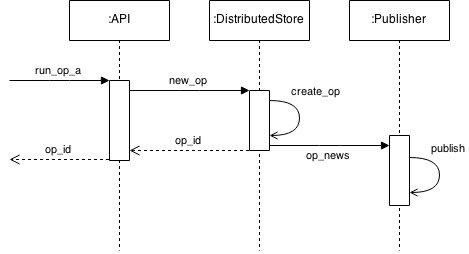
\includegraphics[width=4in]{poster/figures/kseq.png}
  \caption[Sequence diagram of receiving a new operation]
   {Steps we take upon receiving a new operation when the desired dataset is not available locally}
\end{figure}

From the above steps two types of signals will be published to other peers. 
Each of them will trigger certain actions. 
First we show the flow will happen upon receiving an operation update message:
\begin{enumerate}
\item An operation update signal is received.
\item Update our internal operation store silently (without distributing this change).
\end{enumerate}

Next one is a delegate message:
\begin{enumerate}
\item A delegate signal is received.
\item If we have desired dataset do these, otherwise do nothing:
  \begin{enumerate}
  \item Run desired operation on the dataset
  \item Store the result dataset in dataset store \# Currently we choose a random peer to store results there
  \item Add the result dataset id to the operation \# Will be distributed
  \item Update the operation state \# Will be distributed
  \end{enumerate}
\end{enumerate}

\subsection{Scenario 2 - linear operation with two input sets}
First lets have another look at our data distribution and peers as described in analysis chapter:

\begin{tabular}{ l c r }
\em{Server ID} & \em{ Dataset ID} & \em{ Client} \\
S0 & --- & Yes \\
S1 & DS1 & No \\
S2 & DS2 & No \\
\end{tabular}\\

The S0, in this case, is the peer who receives the command and initiates the request. 
Each of the other two peers, S1 and S2, has one of the required datasets, but not both of them. 

In order to realize this scenario we apply \textbf{divide and conquer} and \textbf{produce-consume-collect} methods
as described earlier in this chapter. Then we create one meta operation and two subs. Sub operations will operation exactly as described in previous section
and their results will be reflected in our distributed stores.

As an example we assume that in this case we have two arrays, each consisting of \(10^6\) random numbers. 
We have to first transform these datasets into a set of [0 or 1] based on the number being even or odd (use case 1) 
and then we make a third dataset which contains the sum of every two corresponding numbers in range of [0 to 2].
(in our prototype we have implemented this)

\begin{itemize}
\item Note: in this case each pear is able to run the requested linear operation on one or more datasets.
\end{itemize}

The notation of above mentioned approach will be like this:

%\[ Operation(A + B) = Operation(A) + Operation(B) \]
\[ f(a + b) = f(a) + f(b) \]

In order to run this operation in a collective way, 
we need to think of the type of service calls in our system, 
whether they are blocking or non-blocking. 
Since often the operations in HPC environments are time consuming and long-running, 
we consider the non-blocking approach. 
The operation will be \textbf{submitted} to the collaborative network and
the system decides where and how to store result of an operation (a dataset).
This allows us to design our system in a decentralized way, 
where each peer will inform others (neighbors) about a request using \textbf{publish-subscribe} pattern, 
where the peer will publish a request and the peer which contains 
the dataset will react to the published request and will run the operation. 
All the other peers who do not have the requirements (the dataset for now) will ignore it.
As described for first scenario, 
they will store the details of running operations.


For this operation the following steps will take place on the receiving peer:
On the receiver machine:
\begin{enumerate}
\item If operation requires two dataset continue, otherwise go to next scenario.
\item Store the operation along with input dataset names in the distributed operation store and get the id
\item Create sub commands for each dataset and update the operation store
\item Setup parent operation id for sub-operations
\item Randomly choose one of sub-operations as collector peer (with setting an extra parameter)
\item \textit{Self-launch} the sub operations - This will resemble scenario 1
\item Return operation id to user
\end{enumerate}


For other peers there is only one change while updating an operation:
\begin{enumerate}
\item An operation update signal is received.
\item Update our internal operation store silently (without distributing this change).
\item If we are assigned as collector of this operation do these:
  \begin{enumerate}
  \item Find the parent of this operation
  \item Check state of its sub-operations
  \item If sub-operations are done do these:
    \begin{enumerate}
    \item Download the result of sub-operations to this machine \# Results are small in size
    \item Run the parent operation on them
    \item Store the result and update the operation store
    \end{enumerate}
  \end{enumerate}
\end{enumerate}

\begin{itemize}
\item With the use of operation ids we eliminate the need to get a 
result dataset name from user but we still can accept \textbf{tags} from users.
\end{itemize}

\begin{itemize}
\item We assume every operation involving more than one dataset is made of
other operations which are already defined in the system.
\end{itemize}

\begin{figure}[h]
  \centering
  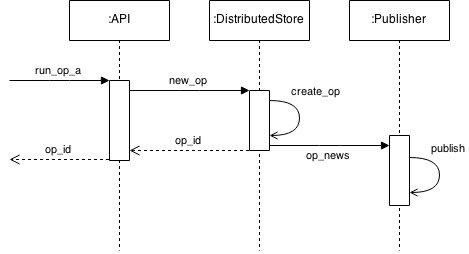
\includegraphics[width=4in]{poster/figures/kseq.png}
  \caption[Sequence diagram showing arrival of an operation message]
   {When a peer is notifed about an operation when it has the desired dataset}
\end{figure}

\subsection{Realizing queries}
Having an operation id at hand a user can query the result of operations. 
Since each peer has enough information about the running operations it can return list of operations and list of datasets.
So user can get informed about current operations and existing datasets and query for operation results or further details.

When user provides an id we return the operation details, such as sub-operation ids, state of each operation,
duration, parent operation id (in case this operation is a child), operation name (the requested service), 
result dataset id, submit time and etc.

Providing a dataset's id we can return the dataset or \textit{download} and store it in a local file to be observed by user.
We discuss more on possible extensions in further works section.
